\documentclass{article}
\usepackage[utf8]{inputenc}
\usepackage{fullpage}
\usepackage{comment}
\usepackage{titlesec}

\setcounter{secnumdepth}{4}
\renewcommand{\baselinestretch}{1.3} 

\title{
	\Huge{\textbf{myTaxiService}}
	\newline
	\huge{\textbf{R}equirement \textbf{A}nalysis and \textbf{S}pecification \textbf{D}ocument}
}
\author{
	Monica Magoni 854091
	\\
	Alberto Cibari 852689
}
\date{October 2015}

\begin{document}

	\maketitle
	\newpage
	\addtocontents{toc}{~\hfill\textbf{Page}\par}
	\renewcommand*\contentsname{\Huge{Summary}}
	\tableofcontents
	
	\newpage
	
\section{Introduction}
	
	\subsection{Purpose}
	This document represents the Requirements Analysis and Specification Document (RASD).
Its aim is to capture all the functional and non-functional requirements that the system-to-be has to respect, in order to satisfy the stakeholders goals, under certain domain properties. This document is also a valid basis for system testing, verification and validation.
	
	\subsection{Scope}
	The aim of our project is to optimize the taxi service of a large city. 
Passengers, once registered to the application, will have the possibility to request a taxi through either the web application or the mobile application. When a request from a passenger arrives, the system-to-be will be able to look for an available taxi (through a fair management of the taxi queue) and send to the passenger the code of the incoming taxi and the waiting time. Taxi drivers will inform the system of their availability and confirm a certain call thanks to a mobile application.
\newline
If the first taxi of the queue is not available, the system will forward the request to the second taxi of the queue and put the first taxi in the last position of the queue. This process will continue until the system finds an available taxi, in order to satisfy the passenger's request.
\newline
Our system will also offer some programmatic interfaces for the development of additional functions, such as taxi sharing.
\newline
The system offers interfaces (APIs) to enable the developement of new services.
\newline
One of these services is the 'Taxi Sharing' option.
It will allow passengers to reserve a taxi in advance, by specifying the origin and the destination of their journey. The reservation must occur at least two hours before the ride and the system will inform the taxi driver ten minutes before the scheduled time.
	
	\subsection{Actors}
	The actors of our system are:
\begin{itemize}
	\item \textbf{Guest}: a person who is not registered in the system. He can not use the features of the system until he registers. 
	\item \textbf{User}: a person who is already registered in the system that uses the application to request or reserve a taxi.
	\item \textbf{Taxi Driver}: a person registered in the system that uses the application to inform the system of the call they take care of and to notify their availability.
	\item \textbf{Administrators}: managers of the web and mobile applications. They manage internally the system and try to fix errors in case of system fault.
\end{itemize}
	
	\subsection{Definitions, acronyms, abbreviations}
	\subsubsection{Definitions}
	In order to avoid confusion, we want to specify the definition of some words that will be often used in our documentation of the project. 
	\begin{itemize}
		\item PASSENGER: for passenger we mean a person, already registered in the system, who has requested or reserved a taxi either through the web or the mobile applications.
		\item USER: a person who is already registered in the system that can use the application to request or reserve a taxi.
		\item GUEST:  a person who is not registered in the system.
		\item REQUEST: message sent by the user's application to the system in order to require a taxi or make a reservation.
		\item CALL: a task received by the taxi drivers after a user made a request.
		\item TAXI ZONE: for taxi zone we mean a zone that is approximately of 2km2. Each taxi zone has a queue of taxi associated. 
		\item QUEUE: for queue we mean the list of taxi available at a specific moment in a certain zone.
		\item NOTIFICATION: for notification we mean a message that could be send by the system to the user (in order to notify the taxi identifier that will satisfy his request and the waiting time) or by the system to a specific taxi driver (in order to notify that a user has a request or a reservation to satisfy).
		\item RESERVATION: the action of the user to book a taxi followed by a request to the system.
		\item TAXI SHARING: the service that allows passengers to share a taxi.
	\end{itemize}

\subsubsection{Acronyms}
	\begin{itemize}
	    \item RASD: Requirements Analysis and Specification Document.
		\item GPS: Global Positioning System.
		\item DBMS: Database Management System.
		\item SD: Sequence Diagram.
	\end{itemize}
	
	\subsection{Stakeholders}
	Compagnie di taxi che lavorano per il comune, il comune stesso.
	
	\subsection{Reference documents}
	\begin{itemize}
	\item Specification Document: Software Engineering 2 Project, AA 2015-2016 Assignments 1 and 2.
	\item IEEE Std 830-1998: IEEE Recommended Practice for Software Requirements Specifications.
\end{itemize}

	\subsection{Overview}
	Our document is organized in four main parts:
\begin{itemize}
	\item Introduction: in this section, we give an overview of the scope and goals of our system-to-be. We also identify the main actors that will be involved in our system and give the basic definitions of some words we will often use in this document.
	\item Overall description: in this part, we try to focus our attention on constraints and assumptions concerning our system-to-be and the world around it. This section also considers some possible future implementations that could be added to our system.
	\item Specific requirements: this section is the body of our document. All the specific requirements that our system need are described here and they are associated with different kinds of diagrams, in order to create a model of the real system.
	\item Bibliography: in this part we specify the documents or books we have referred to.
	
\end{itemize}
	
	
\newpage
\section{Overall Description}

	\subsection{Product perspective}
	The product is a web based application that interacts with a back-end server that handles the data and stores it into a DBMS.
The client application is supposed to be developed in both web and mobile form.
The following are the main features that are included in myTaxiService:
\begin{itemize}
    \item Multi-platform: the back-end system can be used to develope the mobile and web applications.
    \item User account: the system allows the user to create their accounts in the system and provide features of updating and viewing profiles.
    \item Number of users being supported by the system: Though the number is precisely not mentioned but the system is able to support a large number of online users at a time.
    \item Taxi reservation: the system allows the reservation of a taxi, giving the priority of using that taxi to the user  who made the reservation, instead of those who made only a request.
\end{itemize}
	
	\subsection{User characteristics}
		We expect that our user's application will be installed by users who are looking for an easy way to request or reserve a taxi and have the possibility to check their reservations whenever they want.
	The system is developed in order to make the user feel the same experience on both the web and the mobile applications with a similar look.
	\newline
	We expect that our taxi drivers' application will be used by taxi drivers in order to simplify their job: our system will offer a simple way to accept or deny a request and to share taxi drivers' locations.
	
		\subsection{Product functions}
	The main function of the system is to allow users to make a request or a reservation for a taxi and taxi drivers to take care of a specific request.
This is a list of the main actions that our system will provide:

\begin{itemize}
    \item Users:
        \begin{itemize}
        	\item Sign up into the system.
        	\item Log into the system.
        	\item Request a taxi.
        	\item Reserve a taxi.
        	\item Delete requests or reservations.
        	\item Visualize information about requests or reservations.
        	\item Manage their account.
        \end{itemize}
    \item Taxi drivers:
        \begin{itemize}
        	\item Sign up into the system.
        	\item Log into the system.
        	\item Receive information from the system about the city's area they have to cover.
        	\item Notify the system of their availability.
        	\item Receive requests and reservations from the system.
        	\item Accept or decline requests.
        	\item Manage their account.
        \end{itemize}
\end{itemize}

\newpage
\subsubsection{Use Case diagram}
From the list of actions described above, we can derive a Use Case Diagram of our system.

\begin{figure}[h]
    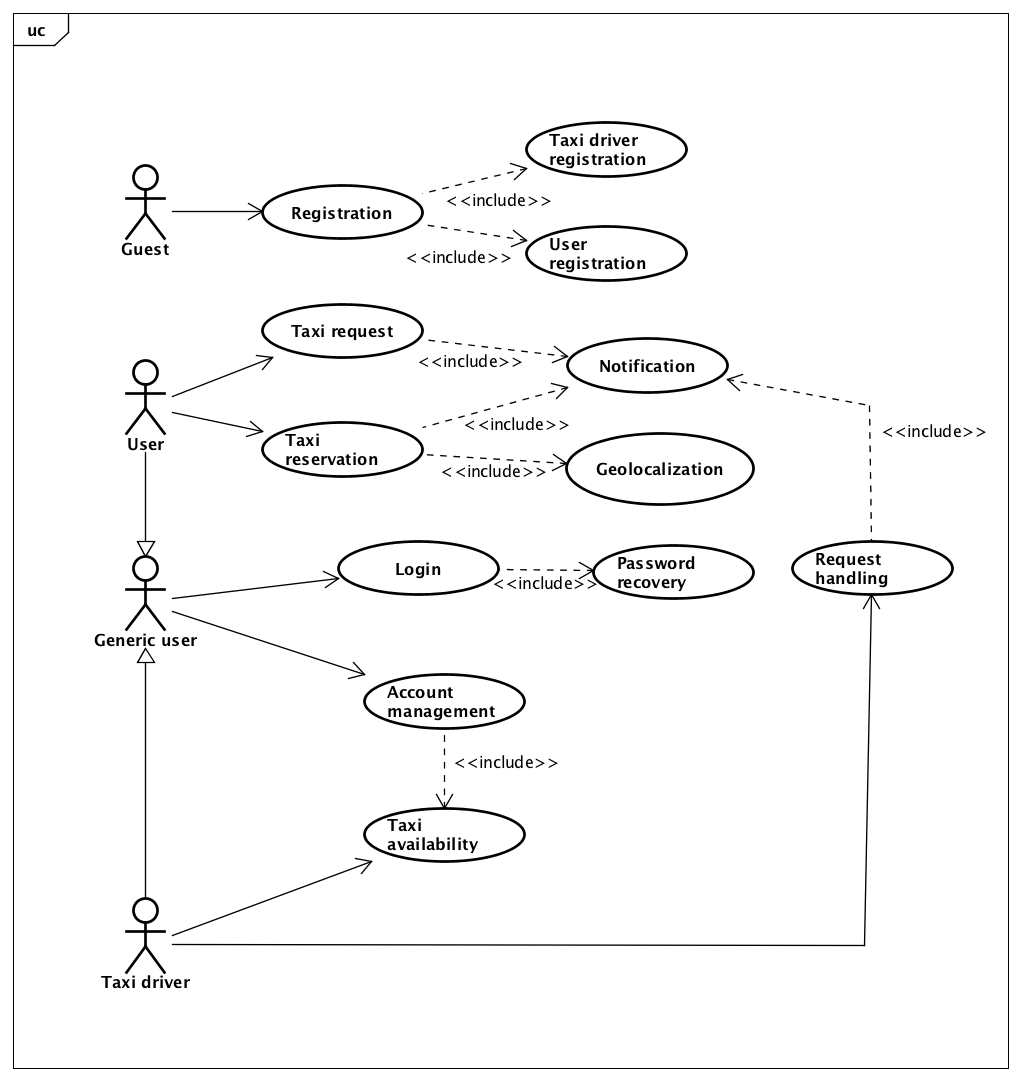
\includegraphics[width=11cm]{./Diagrams/UseCaseDiagram.png}
    \centering
\end{figure}
Figure 1.1: Use Case diagram

	
	\subsection{Assumptions and Dependencies}
	\begin{itemize}
	\item The taxi queue of each area has a maximum length.
	\item If in a specific taxi queue there are too many taxi,  
	the system must reschedule all the taxi's positions.
	\item If in a specific taxi queue there are too few taxi,  
	the system must reschedule all the taxi's positions.
	\item Priority to reservations.
	\item Users can delete reservations within 10 minutes from the appointment. 
	\item Taxi cars are provided of GPS and each of them is associated to a specific taxi identifier.
	\item Taxi drivers can delete accepted requests by contacting administrators, only if there is a problem to their car.
	\item The origin of every reservation must be within the boundaries of the city.
	\item The destination chosen by the passenger must be within 10Km from the city boundaries.
	\item If there are no taxi in a city zone for more than 30 minutes, the system will do a reschedule of the taxi's positions.
	\item Each time a user makes a reservation, he must specify the origin  of the ride.
	\item If a taxi driver doesn't accept/deny a request received by the system within 1 minute, the system forwards the request to the next taxi driver in the queue.
	\item Once a taxi driver accepts a request, the system will delete its identifier from the queue.
\end{itemize}
	
	\subsection{Constraints}
	\subsubsection{Regulatory policies}
	\begin{itemize}
		\item The system must work under the local laws and policies.
		\item The system must ask the user to acquire, store and process personal data. 
	\end{itemize}
	
\subsubsection{Hardware limitations}
	\begin{itemize}
		\item Taxi must have implemented a GPS device in order to track their car's location.
		\item Taxi driver and users must have a mobile device with the mobile application 'myTaxiService' installed. The minimum requirements for the application to be used are: 
		\begin{itemize}
			\item 3G connection
			\item 512MB of RAM
			\item 50MB of free disk space
		\end{itemize}
		\item The web version of the application must work with the versions of IE, Chrome, Opera and Firefox released after 2010.
	\end{itemize}

\subsubsection{Performance requirements}
	\begin{itemize}
		\item The system must reschedule the taxi positions within 5 minutes.
		\item The system must send the user's requests to the taxi drivers as soon as they are received.
		\item If a request arrives during the rescheduling process, the system must use the taxi configuration as it was before the reschedule.
	\end{itemize}

\subsection{Reliability requirements}
	\begin{itemize}
		\item The system must have a minimum availability of 97\%.
		\item The system can be shut down for maintenance only during night time for at least 5 hours a month.
	\end{itemize}

\subsubsection{Security considerations}
	\begin{itemize}
		\item The origin and destination of a user request must be kept secret.
	\end{itemize}

\subsubsection{Interfaces to other applications}
	\begin{itemize}
		\item At the moment 'myTaxiService' has no interfaces with other applications. Possible implementations in the future.
	\end{itemize}

\subsubsection{Parallel operations}
	\begin{itemize}
		\item 'myTaxiService' must support parallel operations from different users when working with database and with all operations done by the user after connection.
	\end{itemize}
		
	\subsection{Future possible implementation}
	\begin{itemize}
	\item An additional service that could be integrated to our mobile application or web application is taxi sharing. This feature allows the passengers who wants to go to the same city area to share the taxi.
	\item Another useful function that could be added to our user's application is the possibility to pay via mobile after the taxi reaches his destination.
	In this way, the system will need to be interconnected to a bank's application.
\end{itemize}
	
	
\newpage	    
\section{Specific Requirements}

	\subsection{External Interface Requirements}
	\subsubsection{Hardware Interfaces}
	The mobile version of the application for taxi drivers must provide a connection to the GPS device installed into the taxi.
	
\subsubsection{Software Interfaces}
	servizi condivisi da web application e mobile applications
	\begin{itemize}
		\item DBMS: \newline
		- SQL Server 2014.
		\item Application server: \newline
		- Windows Server 2012 R2 based on technology .NET.
		\item Operating System (OS): \newline
		- The web application must be able to run on any SO using any browser (IE, Chrome, Opera and Firefox) released after 2010. \newline
		- The mobile applications must be available for devices running Android and iOS.
	\end{itemize}
	
\subsubsection{Communication Interfaces}
	The client application communicate with the back-end server via HTTPS (port 443)
	The back-end services talk with the Microsoft Server DBMS on the default port.
	
	\subsection{System Functions}
	\subsubsection{Guest Registration}
Guests can subscribe to the system via mobile or web application. In both cases they have to fill a form with their personal data and authorize the recipient to use and process their personal details.
If the guest accepts the conditions then he can complete the registration, otherwise it is canceled.
Once a guest is registered, the system checks the consistency of the data inserted by the guest and if everything is correct a mail is sent to the new user. \newline
The registration can also be done by taxi drivers and by a generic user of the service. Taxi drivers must complete the form with more specific data.

	\subparagraph{Functional requirements}
	\noindent
		\begin{itemize}
			\item  During the registration phase guests must choose which kind of account to create: user or taxi driver.
			If the account is a user account then guests must provide:
			\begin{itemize}
				\item Name and surname
				\item Email address
				\item Username
				\item Password
				\item Phone number
			\end{itemize}
			If the account is a taxi driver account, the guest must provide the same information of a user account, with in addiction:
			\begin{itemize}
				\item Taxi Licence ID
			\end{itemize}
			\item The username must be an alphabetic string.
			\item The password must be an alphanumeric string with at least a number and a uppercase character.
			\item The password's length must be between 8 and 16 characters.
			\item There can not be two accounts with the same e-mail and of the same type (user, taxi).
			\item The username is case-insensitive.
			\item Before sending the registration form, the guest will be asked to accept the terms and conditions contract.
		\end{itemize}


\subsubsection{User login/taxi driver login}
Users must be logged in the system to use its services.
During the login process users must choose the type of account (user or taxi), insert the username and the password. If everything is fine, then the users are redirected to their homepage.
In the 'user login' page, guests can be redirected to the 'registration' page.

	\subparagraph{Functional requirements}
	\noindent
		\begin{itemize}
			\item In the 'user field', users can insert the email or the username chosen during the registration phase.
			\item If a user makes a mistake while inserting the credentials, a suggestion field in the page pops up, and it will help the user to recover his credentials.
			\item After inserting the password for 3 times, the account freezes and the user receives an e-mail with the instructions to unfreeze the account.
			\item The 'username field' is case insensitive.
			
		\end{itemize}

\subsubsection{User home page/taxi driver home page}  
After the login process, users are redirected to their main page. Here they have the possibility to choose different actions to perform.
For example, they can reset their password, change personal information or delete their account.
If the user who reached this page is a generic user, he can choose the option of creating a request or a reservation.
If the user is a taxi driver, there are others types of actions available: for instance, he can view the pending requests sent by the system and accept or decline them.

	\subparagraph{Functional requirements}
	\noindent
		\begin{itemize}
			\item A generic user can:
			\begin{itemize}
				\item Change password.
				\item Change account information.
				\item Make a taxi request.
				\item Make a Reservation.
				\item Delete requests or reservation.
				\item Visualize all the requests/reservations done.
				\item View the history of all the rides done.
			\end{itemize}
			\item A taxi driver user can:
			\begin{itemize}
				\item Change password.
				\item Change account information.
				\item Delete account.
				\item View the history of all the rides done.
				\item Activate/Deactivate taxi service.
				\item View the pending request.
				\item Track the taxi via GPS.
			\end{itemize}
			
			\item During the 'password changing' phase, the old password should provided with the new one.
			\begin{itemize}
				\item The new password must be an alphanumeric string with at least a number and a uppercase character.
				\item The new password length must be between 8 and 16 characters. 
				\item The new password must be different from the old one.
			\end{itemize}
			\item During the 'account deletion' phase, after the confirmation of the user, a mail is sent to him with a link that allows to deactivate the account.
			\item The deletion account function delete the account but keeps all the user information. The information are kept as history in the DB.
			\item Activate/Deactivate taxi service: the taxi driver use this function to tell the system to activate/deactivate the taxi service adding/removing him from the taxi queues in the city zones.
			\item A request received by a taxi driver is displayed in his main page for one minute, then it is passed to the next user in the city zone queue.
		\end{itemize}


\subsubsection{Activation/deactivation of the taxi services}
When a taxi driver is visiting his home page in the application, he should be able to activate or deactivate his taxi service sending a notification to the system.
When the system receives the notification from the user application about activating/deactivating the taxi system, it checks if the GPS installed in the car connected to the account is on. If there are no errors the taxi is put into a taxi zone queue/removed from the queue. And the system sends him a notification

	\subparagraph{Functional requirements}
	\noindent
		\begin{itemize}
			\item The activation of the service can occur only if the GPS installed on the car is active, otherwise the taxi driver receives an alert on his application.
			\item If the system can not receive the GPS signal every 5 minutes, it sends a notification to the user.
			\item If the system can not receive the GPS signal for more than 20 minutes, the taxi service is deactivated.
			\item The taxi service can be deactivated only if the user isn't taking a request/reservation.
		\end{itemize} 


\subsubsection{Request making}
The user should be able to make a taxi request from the web application and the mobile application. If the request comes from the web application, the user has to tell the system the origin of the ride, otherwise the origin is taken using the GPS of the mobile application.
After the user makes the request, he receives a notification from the system with the identifier of the taxi and the possible arrival time of the taxi.
Once the request is sent to the system, the system has to send it to the first taxi driver available, who can accept or deny the request.

	\subparagraph{Functional requirements}
	\noindent
		\begin{itemize}
			\item If the request is made using the web application, the system shall be provided with the passenger location inserted directly by the user.
			\item If the request is made using the mobile application, the system can use the GPS position to identify the user location.
			\item If the GPS is not available, the system tells the passenger to insert the correct origin location for the taxi ride.
			\item If the origin is not specified (neither from GPS nor from the user insertion), the user can not proceed to send the request.
			\item If a request is not accepted by a taxi driver, it is passed to the next driver in the queue of the city zone.
		\end{itemize}


\subsubsection{Reservation making}
The user should be able to make a taxi request from the web application and the mobile application. The reservation must contain the origin and the destination of the ride. The user has to specify also the date and hour of the reservation. If the values for the reservation are valid, the user can send the request to the system. Then the user will receive a notification with the taxi identifier.

	\subparagraph{Functional requirements}
	\noindent
		\begin{itemize}
			\item The origin and the destination must be valid [View assumptions]. They must be within 10Km from the city boundaries.
			\item If the GPS is available the user can use the current position as origin of the ride.
			\item The date and the time of the reservation must be valid values.
			\item The system does not allow reservation after 24 hours from the current system time.
			\item The system sends a notification to the user 10 minutes before the hour chosen by the user for the ride. The notification contains the taxi identifier.
		\end{itemize}


\subsubsection{Taxi driver notification handling}
After a taxi driver activates the taxi service, he can receive a notification request for a taxi ride. He can accept or refuse the request. If the request is accepted, he has to go to the origin location indicated in the notification.

    \subparagraph{Functional requirements}
    \noindent
        \begin{itemize}
            \item After the taxi driver receives a notification, if the system does not receive an answer within 1 minute, the notification is passed to the following driver in the taxi queue.
            \item If there are no available taxi drivers in a city zone, the system looks for an available taxi for a maximum of 10 times. 
            \item If the system can not find an available taxi, it sends a notification of failure to the user.
            \item When the taxi reaches the origin zone, the system asks him to confirm the begin of the ride.
            \item When the taxi reaches the destination zone, the system asks him to confirm the end of the ride.
            \item After the taxi driver confirms the begin of a ride, the system sets his status to 'busy'.
            \item After the taxi driver confirms the end of a ride, the system sets his status to 'available'.
            \item When a ride is completed, the system stores the data of the ride into the DB.
        \end{itemize}
        
        
\subsubsection{Zone queue handling}
The system has to manage the queue of taxi in all the different city zones. It has to schedule the requests and send them to the right taxi.
    
	\subparagraph{Functional requirements}
	\noindent
	    \begin{itemize}
	        \item The queues use the FIFO policy.
	        \item When a taxi connects to the system and sets its status to 'available', the system insert it into a queue.
	        \item The queue is identified by the GPS positions of the city zones: taxi are put in the queues according to their GPS location.
	    \end{itemize}
    

	
	\subsection{Scenarios}
	\subparagraph{Scenario 1: User Registration}
\noindent
\newline
    Bob is a tourist who just came in Gotham city. He discovers that the city has a system of taxi reservation using a mobile application. So he downloads the mobile app and opens it. The first page presented is the login page, but he hasn't an account yet. So he taps the registration button and he is redirected to the registration page. There he inserts his name and surname, his email and his username and password. He decides to leave the address and phone fields empty.
    Before sending the registration form, he accepts the terms and conditions contract, and sends the registration.
    After a while he receives a mail with a link for the confirmation of the account creation.

\subparagraph{Scenario 2: Taxi driver registration}
\noindent
\newline
    Alice is a taxi driver. She wants to participate in the city government project 'myTaxiService'. At her home she enters her browser in the main page of the myTaxiService web site. She isn't registered yet, so the click on the registration button that redirects her to the registration page. Here she enters her personal data, her username, password, and her taxi licence ID. Once filled the registration form, she accepts the terms and conditions of the service and submits the registration. A confirmation mail is sent to her with a link to complete the registration. She clicks it and she is redirected to the login page.

\subparagraph{Scenario 3: User login}
\noindent
\newline
    Charlie has to go to the airport for his holiday trip. At home on his web browser he enters the myTaxiService site. In the login page he enters his username and password, chosen during the registration phase. Once entered correctly the required values, he clicks the login button and visualizes his home page.

\subparagraph{Scenario 4:User login error}
\noindent
\newline
    Daniel wants to enter the myTaxiService site to view the log of all the requests he accepted. In the login page he enters his username and password, but unfortunately they are wrong. So he retries again but writes them wrong again.
    So he decides to try the recovery password system. In the login page he clicks on the 'Recovery' button. The system tells him it sents an e-mail with the new password auto-generated for entering the account.
    After Daniel receives the mail, he retries to enter into the system using the new password. After clicking onto the Login button he visualizes his homepage

\subparagraph{Scenario 5: Activation of taxi service}
\noindent
\newline
    Emily is beginning her work day as a taxi driver. She uses the myTaxiService system to handle the requests for a taxi. To enable her taxi to receive request she has to activate the service via myTaxiService application. Once entered her home page, after the login, she clicks the button for the activation. But she receives an alert regarding the GPS signal: "the system can't track the taxi GPS signal. The service can not be activated". So she turns on the GPS device in the car and retries the activation. This time the system finds the GPS signal and activate her service, putting her taxi in the queue of the city zone where che is in.
    
\subparagraph{Scenario 6: Taxi request}
\noindent
\newline
    It's a sunny day and Michael, who loves swimming, decides to go to the open air swimming-pool of his city. Unfortunately, the swimming-pool is quite far from his home and so he decides to make a taxi request. He remembers that some days ago, he registered to the 'myTaxiService' application. So, he logs in from his mobile application and from his home page, he clicks on the button 'make a taxi request'. The GPS on his mobile device is activated and so, after few seconds, he receives a notification containing the taxi identifier, that has been chosen by the system in order to satisfy his request, and the waiting time expected.

\subparagraph{Scenario 7: Taxi reservation}
\noindent
\newline
    Lorena is planning a visit to the local museum of the city. She loves planning every single detail of her trip and so she decides to make a taxi reservation in advance. She opens the web application of 'myTaxiService' and so she logs in. From the home page, she clicks on 'make a taxi reservation'; then, due to the fact that her GPS is not activated, she selects the origin and the destination of her ride. She has also to specify the date and the hour of the ride. After some seconds, she receives a notification from the application that confirms her reservation and indicates the taxi identifier that will take care of her journey.

\subparagraph{Scenario 8: Taxi driver request acceptance}
\noindent
\newline
    Alessia is a taxi driver, already registered in the system, and she is waiting for a request at the parking of city zone 2. She set her status as 'available' from her taxi driver application. Suddenly, she receives a notification on her device: it's a request from a user. She clicks on the button 'accept' and, after viewing where the user is located, she is ready to go to the origin of the ride.
	
	\subsection{Function sequence diagrams}
	\subparagraph{User registration}
\noindent
    \begin{figure}[h]
        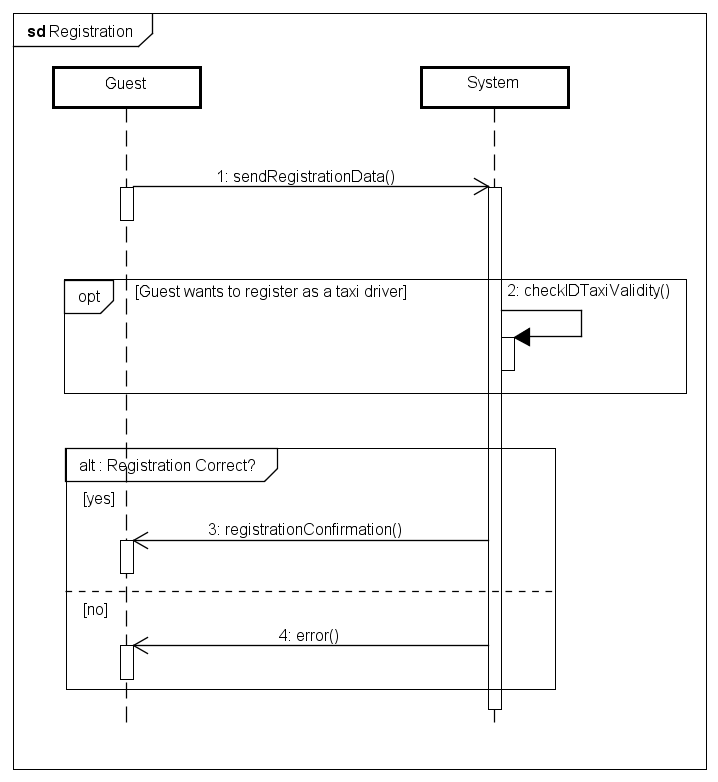
\includegraphics[width=11cm]{./Diagrams/Registration.png}
        \newline Figure 1.2: SD - User registration
        \centering
    \end{figure}
\newpage
\subparagraph{User login}
\noindent
\begin{figure}[h]
        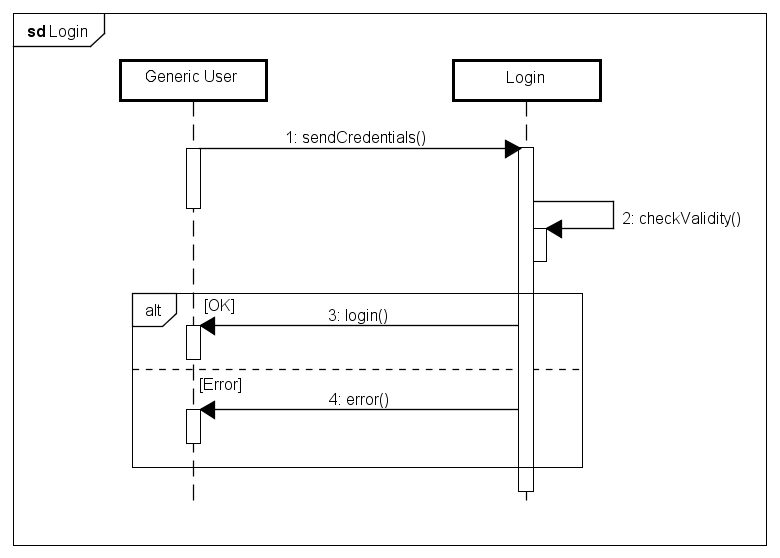
\includegraphics[width=11cm]{./Diagrams/Login.png}
        \newline Figure 1.3: SD - User login
        \centering
    \end{figure}
\noindent

\newpage
\subparagraph{Taxi request}
\noindent
    \begin{figure}[h]
        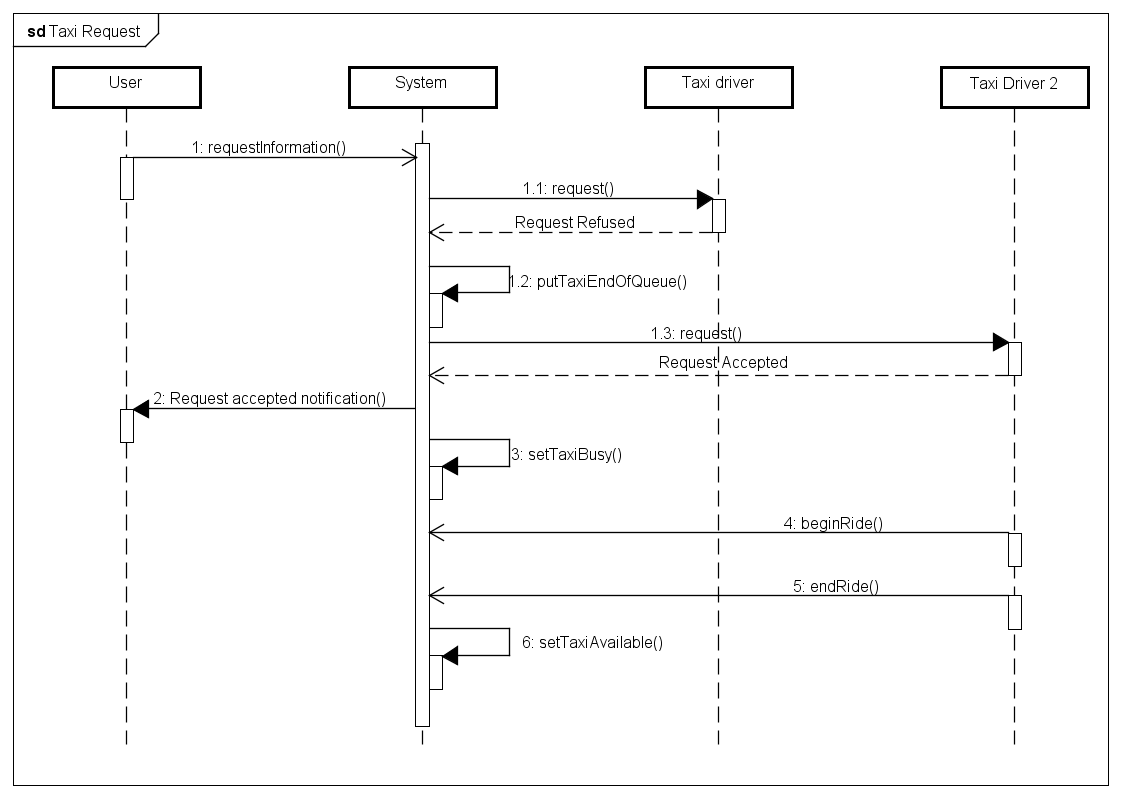
\includegraphics[width=11cm]{./Diagrams/TaxiRequest.png}
        \newline Figure 1.4: SD - Taxi request
        \centering
    \end{figure}
\newpage
\subparagraph{Taxi reservation}
\noindent
    \begin{figure}[h]
        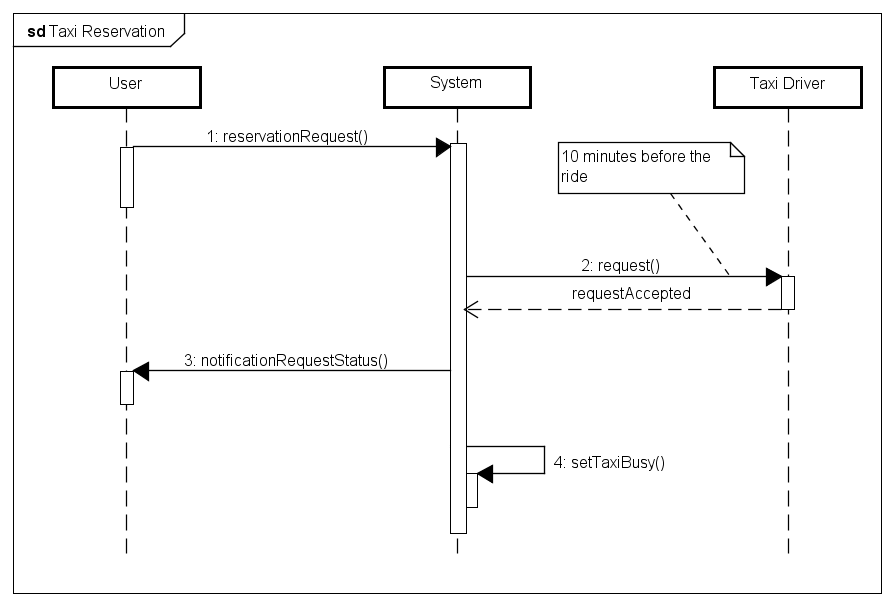
\includegraphics[width=11cm]{./Diagrams/TaxiReservation.png}
        \newline Figure 1.5: SD - Taxi reservation
        \centering
    \end{figure}


	
	\subsection{Non-functional requirements}
	\subsubsection{Performance Requirements}

\subsubsection{Design Constraints}

\subsubsection{Maintainability}

\subsubsection{Security}

	
\end{document}